\documentclass{article}
\usepackage{tikz}

\begin{document}

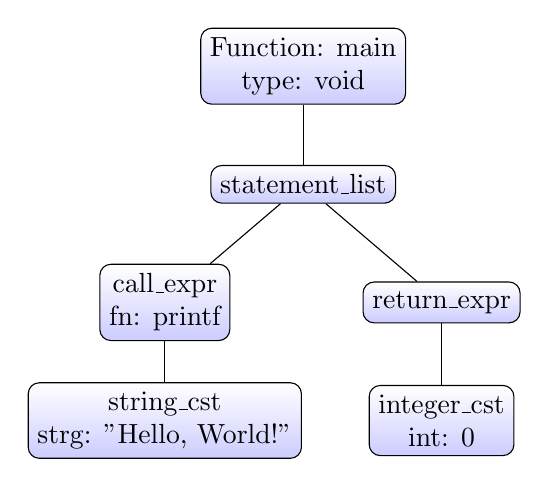
\begin{tikzpicture}[sibling distance=10em,
  every node/.style = {shape=rectangle, rounded corners,
    draw, align=center,
    top color=white, bottom color=blue!20}]]
  \node {Function: main\\type: void}
    child { node {statement\_list}
      child { node {call\_expr\\fn: printf}
        child { node {string\_cst\\strg: "Hello, World!"}} }
      child { node {return\_expr}
        child { node {integer\_cst\\int: 0}} }};
\end{tikzpicture}

\end{document}
